
% region CPBP bar graphs

% Bar graph representing the blue constraint's marginals on variable x
\newcommand{\emptyGraph}{
    \begin{tikzpicture}
        \begin{axis}[
            opacity=0,
            ybar,
            axis y line=none,
            axis x line=bottom,
            axis line style={draw=none},
            ymin=0,
            ymax=100,
            width=2.2cm,
            height=2.2cm,
            bar width=1.5mm,
            xtick={a,b,c,d,e},
            xtick style={draw=none},
            symbolic x coords={a,b,c,d,e},
            xticklabel style={font=\scriptsize, anchor=north, yshift=-2pt},
            axis x line=bottom,
            axis y line=left,
            tick align=inside,
            enlarge x limits=0,
            clip=false,
        ]
            \addplot+[draw=none, fill=none, forget plot] coordinates {(e,100)};
        \end{axis}
    \end{tikzpicture}
}

% Bar graph representing the blue constraint's marginals on variable y
\newcommand{\blueGraphY}{
    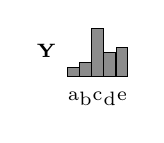
\begin{tikzpicture}
        \begin{axis}[
            ybar,
            axis y line=none,
            axis x line=bottom,
            axis line style={draw=none},
            ymin=0,
            ymax=100,
            width=2.2cm,
            height=2.2cm,
            bar width=1.5mm,
            xtick={a,b,c,d,e},
            xtick style={draw=none},
            symbolic x coords={a,b,c,d,e},
            xticklabel style={font=\scriptsize, anchor=north, yshift=-2pt},
            axis x line=bottom,
            axis y line=left,
            tick align=inside,
            enlarge x limits=0,
            clip=false,
        ]
            \addplot+[fill=gray!90, draw=black] coordinates {
                (a,20) (b,30) (c,100) (d,50) (e,60)
            };
            \node[
                anchor=south east,
                font=\scriptsize\bfseries,
                xshift=-1mm, yshift=-5mm
            ] at (current axis.north west) {Y};
        \end{axis}
    \end{tikzpicture}
}

% Bar graph representing the red constraint's marginals on variable w
\newcommand{\redGraphW}{
    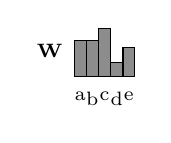
\begin{tikzpicture}
        \begin{axis}[
            ybar,
            axis y line=none,
            axis x line=bottom,
            axis line style={draw=none},
            ymin=0,
            ymax=100,
            width=2.2cm,
            height=2.2cm,
            bar width=1.5mm,
            xtick={a,b,c,d,e},
            xtick style={draw=none},
            symbolic x coords={a,b,c,d,e},
            xticklabel style={font=\scriptsize, anchor=north, yshift=-2pt},
            axis x line=bottom,
            axis y line=left,
            tick align=inside,
            enlarge x limits=0,
            clip=false,
        ]
            \addplot+[fill=gray!90, draw=black] coordinates {
                (a,75) (b,75) (c,100) (d,30) (e,60)
            };
            \node[
                anchor=south east,
                font=\scriptsize\bfseries,
                xshift=-1mm, yshift=-5mm
            ] at (current axis.north west) {W};
        \end{axis}
    \end{tikzpicture}
}

% Bar graph representing the combined marginals on variable x
\newcommand{\combinedX}{
    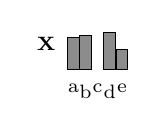
\begin{tikzpicture}
        \begin{axis}[
            ybar,
            axis y line=none,
            axis x line=bottom,
            axis line style={draw=none},
            ymin=0,
            ymax=100,
            width=2.2cm,
            height=2.2cm,
            bar width=1.5mm,
            xtick={a,b,c,d,e},
            xtick style={draw=none},
            symbolic x coords={a,b,c,d,e},
            xticklabel style={font=\scriptsize, anchor=north, yshift=-2pt},
            axis x line=bottom,
            axis y line=left,
            tick align=inside,
            enlarge x limits=0,
            clip=false,
        ]
            \addplot+[fill=gray!90, draw=black] coordinates {
                (a,65) (b,70) (d,75) (e,40)
            };
            \node[
                anchor=south east,
                font=\scriptsize\bfseries,
                xshift=-1mm, yshift=-5mm
            ] at (current axis.north west) {X};
        \end{axis}
    \end{tikzpicture}
}

% Bar graph representing the combined marginals on variable z
\newcommand{\combinedZ}{
    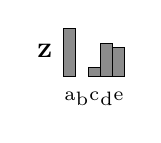
\begin{tikzpicture}
        \begin{axis}[
            ybar,
            axis y line=none,
            axis x line=bottom,
            axis line style={draw=none},
            ymin=0,
            ymax=100,
            width=2.2cm,
            height=2.2cm,
            bar width=1.5mm,
            xtick={a,b,c,d,e},
            xtick style={draw=none},
            symbolic x coords={a,b,c,d,e},
            xticklabel style={font=\scriptsize, anchor=north, yshift=-2pt},
            axis x line=bottom,
            axis y line=left,
            tick align=inside,
            enlarge x limits=0,
            clip=false,
        ]
            \addplot+[fill=gray!90, draw=black] coordinates {
                (a,100) (c,20) (d,69) (e,60)
            };
            \node[
                anchor=south east,
                font=\scriptsize\bfseries,
                xshift=-1mm, yshift=-5mm
            ] at (current axis.north west) {Z};
        \end{axis}
    \end{tikzpicture}
}

% endregion

    
\begin{tikzpicture}[node distance=10pt and 20pt, thick]
    % Left side: stacked bar plots with labels
    \matrix (left)[
        matrix of nodes,
        nodes={anchor=west},
        row sep=10pt,
        inner sep=0pt
    ] {
        \node {\emptyGraph}; \\
        \node {\blueGraphY}; \\ 
        \node {\emptyGraph}; \\
    };
    % Draw blue bounding box around left matrix
    \node[draw=blue, thick, inner sep=5pt, fit=(left)] (blueBox) {};

    % Right side: same matrix as left, shifted right of middle
    \matrix (right)[
        matrix of nodes,
        nodes={anchor=west},
        row sep=10pt,
        inner sep=0pt,
        right=4cm of left.center
    ] {
        \node {\emptyGraph}; \\
        \node {\redGraphW}; \\
        \node {\emptyGraph}; \\
    };
    % Draw red bounding box around left matrix
    \node[draw=red, thick, inner sep=5pt, fit=(right)] (redBox) {};
    
    % Right side: same matrix as left, shifted right of middle
    \matrix (middle)[
        matrix of nodes,
        nodes={anchor=west},
        row sep=10pt,
        inner sep=0pt,
        right=1.5cm of left.center
    ] {
        \node {\combinedX}; \\
        \node {\emptyGraph}; \\
        \node {\combinedZ}; \\
    };

    \node[draw=green, dashed, inner sep=5pt, fit=(left)(right)] (greenBox) {};
\end{tikzpicture}
